The user here provides information about the building and the units
the user will work in. The widget itself presents 3 separate frames,
as shown in \autoref{fig:figure2}, to the user:

\begin{enumerate}
\item Building Information frame in which user provide general information about the building, this include year of construction and type.
\item Properties frame in which user provides information about number of stories, width, depth, plan area and height of the building.
\item Location frame in which user provides location of the building. This information is used in some of event widgets to obtain events specific to the building.
\item Units frame  in which user specifies what the units will be for the inputs and outputs. Some widgets will require inputs in different units. These entries will contain units beside the specific entry to mark this.
\end{enumerate}


\begin{figure}[!htbp]
  \centering {
    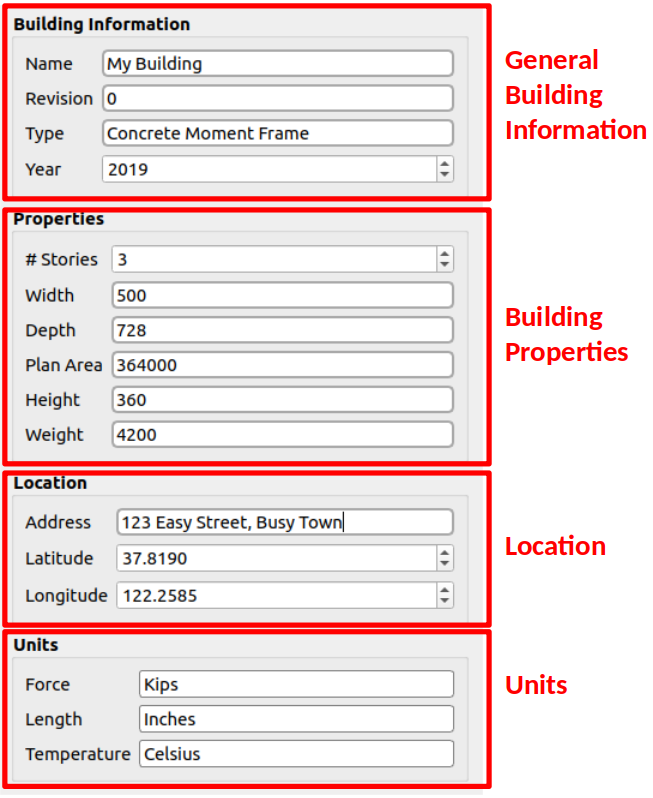
\includegraphics[width=0.5\textwidth]
    {usage/figures/gi.png} }
  \caption{BIM}
  \label{fig:figure2}
\end{figure}

